\documentclass{article}
\usepackage{amssymb}
\usepackage{amsmath}
\usepackage{multicol}
\usepackage{graphicx}
\usepackage{amsthm}
\usepackage{verbatim}
\usepackage{color}
\usepackage[dvipsnames]{xcolor}
\usepackage{tikz}


\oddsidemargin 0.0 in
\textwidth 6.5 in
\topmargin 0.0 in
\headheight 0.0 in
\headsep 0.0 in
\textheight 8.75 in
\makeatletter



\marginparwidth 40pt %  Width of marginal notes.
\marginparsep 10pt %    Horizontal space between outer margin and note.
\newcommand{\con}{\vee}
\newcommand{\dis}{\wedge}


\begin{document}
%\maketitle 

\begin{center}
    {\bf Thermodynamic Power Cycle Analysis: A Crash Course}\\
    Jackson Harvey, RF Technology Group\\
    11/11/2022\\
\end{center}


%%
\vspace{0.1in}
\noindent{\bf DEFINITION OF VARIABLES}  \\
\noindent{\bf Operational Parameters}
\begin{flalign*}
    P & : \mbox{Pressure} & \\
    T & : \mbox{Temperature} \\
    u & : \mbox{Internal Energy} \\
    s & : \mbox{Entropy}
    ke & : \mbox{Kinetic energy}\\
    pe & : \mbox{Potential}\\
    V & : \mbox{Velocity}\\
    g & : \mbox{Gravitational Acceleration}
\end{flalign*}
\noindent\mbox{\bf Fluid Properties}
\begin{flalign*}
    c_p,c_v & : \mbox{Specific heat at constant pressure ($c_p$) and constant volume ($c_v$)} & \\
    k       & : \mbox{Ratio of specific heats},      k = c_p/c_v                                \\
    R       & : \mbox{Gas Constant for substance}, R = c_p-c_v = R_u/M                          \\
    \rho    & : \mbox{Density}                                                                  \\
    v       & : \mbox{Specific Volume}                                                          \\
    M,R_u   & : \mbox{Molar mass ($M$) and universal gas constant ($R_u$)}                      \\
\end{flalign*}
\begin{enumerate}
    \item{PRELIMINARIES}\\
    The fundamental equations associated with thermodynamics are known and well documented. 
    The purpose of this paper is not to rederive these relationships, 
    therefore, a certain level of familiarity with thermo is assumed for the reader. 
    Nonetheless, this section presents several useful and neccesary relationships used throughout the report.
    \begin{enumerate}

        \item{NOTATION} \\ 
        In the majority of this report energy will be conveyed in {\bf Unit Mass Form}, also known as "specific" form. 
        The Total Energy, $E$ [kJ], and specific energy, $e$ [kJ/kg],  are related by: $e = E/m$, where m is the mass [kg]. 
        Similairly, often energy is expressed in time-rate form ($d/dt$) which is denoted by: $\frac{d}{dt}E = \dot{E}$ [kW].
        $\dot{E}$ and $e$ are related by $\dot{E}=\dot{m}e$, where $\dot{m}$ is the mass flow rate in [kg/s].

        \item{THERMODYNAMIC PROPERTIES} \\
        This section provides a brief review of thermodynamic properties and their implications.\\

        {\bf Intensive Properties} are the mass-independent properties of a system $(T,P,\rho)$. 
        These properties cannot be put into into "specific" form as the relationship is meaningless. \\

        {\bf Extensive Properties} are characterstic properties that depend on the system configuration.
        Meaning they are not innate to the fluid, rather a product of the conditions. 
        Some examples of these proprties are $E$ and volume $\mathbb{V}$. These properties can be put into into
         "specific" form as they are a function of mass, and therefor of the form
        $X = mx$, wher $X$ is the total properties and $x$ is the specific property. 
        It should also be noted that the specific volume $\nu = \frac{\mathbb{V}}{m} = \frac{1}{\rho}$\\

        \emph{**In the remaining sections of the paper, any reference to $V$ is velocity while $\mathbb{V}$ is volume}

        \item{KEY RELATIONSHIPS}\\
        First we review the definition of the {\bf Total Differential, }$df$, of some function $f(x,y)$\\
        \begin{equation}
            df = \left(\frac{\partial f}{\partial x}\right)_ydx + \left(\frac{\partial f}{\partial y}\right)_xdy
        \end{equation}
        We should also introduce the definition of enthalpy\\
        \begin{equation}\label{enthalpy}
            h = u + Pdv
        \end{equation}
        
        the gibbs relationships\\
        \begin{equation}\label{gibbs}
            \begin{aligned}
            Tds &= du + Pdv\\
            Tds &= dh - vdP
        \end{aligned}\end{equation}
    %%%%%%%%%%%%%%%%%%%%%%%%%%%%%%%%%%%%%%%%%%%%%%%%%%%%%%%%%    
        We now take the time to further evaluate two special cases relevant to power cycles.
        \begin{enumerate}
            \item{Incompressible Substances}\\
                By nature of incompressible substances\\
                \begin{equation*}
                    \begin{aligned}
                    \nu = \text{constant } \to dv &= 0\\
                    c_p(T) = c_v(T) &= c(T)\\
                    du &= c(T) dT
                    \end{aligned}
                \end{equation*}
                From the definition of enthalpy in Eq \ref{enthalpy}, we can say:
                \begin{equation}
                    dh = c(T)dT + \nu dP
                \end{equation}
            %%%%%%%%%%%%%%%%%%%%%%%%%%%%%%%%%%%%%%%%%%%%%%%%%%%%%%%%%  
            \item {Ideal Gas}\\
                Intuitively, the first equaton nececarry to evaluate an ideal gas is the ideal gas law:
                \begin{equation}
                    \label{idealGas}
                    \begin{aligned}
                    P\nu=RT
                    \end{aligned}
                \end{equation}
                In addition, we show the specific relationships for an ideal gas:
                \begin{equation}
                    \label{ig_relation}
                    \begin{aligned}
                        c_p &= c_v+R\\
                        k &= c_p/c_v\\
                    du &= c_vdT\\
                    dh &= c_pdT
                \end{aligned}\end{equation}
                Finally, when an ideal gas with \emph{constant specific heats} undergoes an {\bf isentropic} process, we can say:
                \begin{equation}
                    \label{pvt}
                        \left(\frac{T_2}{T_1}\right)_{s=const} = \left(\frac{P_2}{P_1}\right)^{(k-1)/k}=\left(\frac{v_1}{v_2}\right)^{k-1}
                \end{equation}

            %%%%%%%%%%%%%%%%%%%%%%%%%%%%%%%%%%%%%%%%%%%%%%%%%%%%%%%%%  
        \end{enumerate}
    \end{enumerate}


    \item{ENERGY BALANCE}\\
    \begin{figure}[h!]
        \centering
        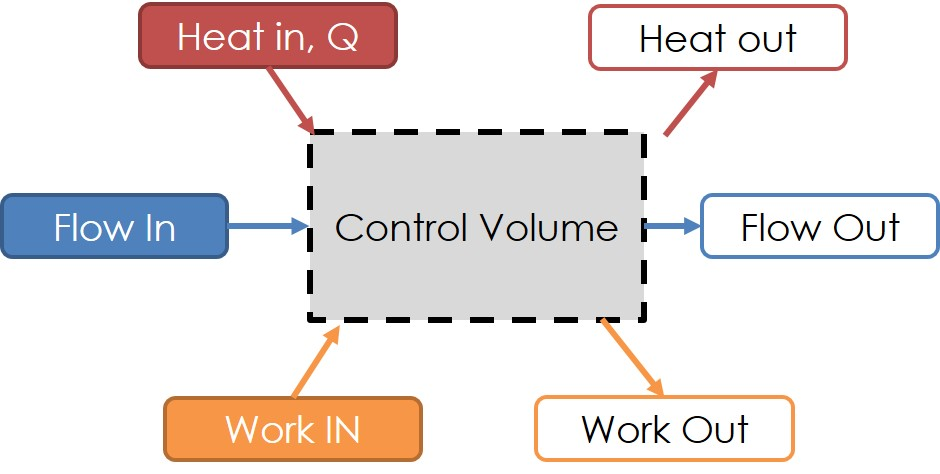
\includegraphics[width=4in]{CV_DIAGRAM.jpg}
        \caption{Control Volume General Diagram}
        \label{cvdiagram}
    \end{figure}
    %%%%%%%%%%%%%%%%%%%%%%%%%%%%%%%%%%%%%%%%%%%%%%%%%%%%
    \begin{enumerate}
        \item{Energy Transport by Mass}
            \begin{equation}
                \theta  = h + ke + pe = h + \frac{V^2}{2} + gz
            \end{equation}
    %%%%%%%%%%%%%%%%%%%%%%%%%%%%%%%%%%%%%%%%%%%%%%%%%%%%
        \item{Total Energy of Flowing Fluid}
            \begin{equation}
                \begin{aligned}
                    E_{mass}        &= m\theta      \textit{  (Amount)}\\
                    \dot{E}_{mass}  &=\dot{m}\theta  \textit{ (Rate)}
                \end{aligned}
            \end{equation}
    %%%%%%%%%%%%%%%%%%%%%%%%%%%%%%%%%%%%%%%%%%%%%%%%%%%%
        \item{\bf ENERGY BALANCE}\\
        \begin{equation}\label{ebalance}
            \begin{aligned}
                \dot{Q}_{in} + \dot{W}_{in} + \sum_{in}\dot{m}\theta &= \dot{Q}_{out} + \dot{W}_{out} + \sum_{out}\dot{m}\theta\\
                \dot{Q}_{net} -  \dot{W}_{net} &= \sum_{out}\dot{m}\theta-\sum_{in}\dot{m}\theta\\
                \textit{Where    }  \dot{Q}_{net} &= \dot{Q}_{in} - \dot{Q}_{out}\\
                \dot{W}_{net} &= \dot{W}_{out} - \dot{W}_{in}
            \end{aligned}
        \end{equation}
    \end{enumerate}
    \item{\bf WORK RELATED COMPONENTS}
    \begin{enumerate}
        \item{Pumps and Compressors}\\
        Pumps and compressors are components which convert external work into flow work by increasing the pressure and of the working fluid.
        It is standard to assume $\dot{Q}=\dot{q}=\Delta ke = \Delta pe = 0$ for said components. Furthermore, there is no output component for work, so
        $\dot{W}_{net} = -\dot{W}_{in}$. Equation \ref{ebalance} then reduces to:
        \begin{equation}\label{ebal_pump}
            \begin{aligned}
                \dot{W}_{in} &= \sum_{out}\dot{m}\theta-\sum_{in}\dot{m}\theta\\
                &= \dot{m}(h_{out}-h_{in})
            \end{aligned}
        \end{equation}


        mirror components, the only difference being the working fluid of the circuit.
        Both components require external work input in order to increase the pressure of the working fluid.
        \item{Turbines}
    \end{enumerate}
    \item{\bf HEAT TRANSFER COMPONENTS}
    \begin{enumerate}
        \item{Heat Exchangers}
    \end{enumerate}
\end{enumerate}
\end{document}

%or $x\in\mathbb{N}$, $f(x) = \left\{ \begin{array}{cl} a_x^{1} & x\leq m_1 \\ a_{x-m_1}^2 & m_1<x\leq (m_1+m_2) \\ a_{x-(m_1+m_2)}^3 & (m_1+m_2)<x\leq (m_1+m_2+m_3)\\ ... & ...\\a_{x-(\sum_{i=1}^{n-1}m_i)}^n& (\sum_{i=1}^{n-1}m_i)<x<\sum_{i=1}^{n}m_i) \end{array} \right.  $\\ \\
%$For $a\in A$, $f(a) = \left\{ \begin{array}{cl} 14 & a=x\\ -3 & a=y\\ t & a=\{a,b,c\}\end{array} \right.  $\\ \\